<<<<<<< 748b67fd60b26d45750e10209255345ebe612814
\section{Theorie}
Im diesem Versuch wird der RLC-Schwingkreis untersucht, dieser besteht aus folgenden
Bauteilen: Widerstand $R$, Induktivität $L$ und Kondensator $C$.
Ähnlich zum RLC-Schingkreis ist der RC-Schwingkreis aufgebaut, er bestitzt nur einen
Energiespeicher, den Kondensator $C$. Daher kann der Strom $I$ nur in eine Richtung fließen.
Der RLC-Schwingkreis besitzt zwei Energiespeicher, einen Kondensator und eine
Spule. Wird nun Energie in das System hineingepumt, pendelt diese zwischen Kondensator und
Spule, wodurch der Strom sein Vorzeichen ändert. Der Widerstand, der hier dem
Dämpfungsfaktor entspricht, wandelt einen Teil der Energie in Wärme um. Nach einer
gewissen Zeitspanne ist keine elektrische Energie mehr vorhangen und die Schwingung
kommt zum erliegen. Dieses Verhalten wirdauch als gedämpfte Schwingung bezeichnet.
Wenn kein Widerstand $R$ im System verbaut ist, wird dieses System als
ungedämpften Schwingung bezeichnet.
\begin{figure}[H]
  \centering
  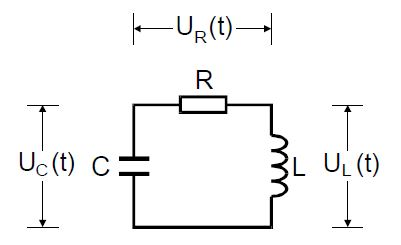
\includegraphics[height=5cm]{RLC.JPG}
  \caption{Darstellung eines RLC-Scwingkreises}
  \cite{skript}.
  \label{fig:RLC}
\end{figure}
Wird an den Schwingkreis von außen eine Spannung angelegt, schwingt dieser
mit der Frequenz der angelegten Spannung. Die so erhaltene Schwingung wird als
ezwungene Schwingung bezeichnet. Hat die von außen angelete Spannung die "richtige"
Frequenz (abhänging vom verwendeten System/Schwingkreis), dann erreicht die Stromamplitude im
Schwingkreis ihr Maximum. Dieser Fall wird als Resonanzfall bezeichnet und tritt bei der
sogenannten Resonanzfrequenz auf.

\subsection{Gedämpfte Schwingung}
In einem RLC-Schwingkreis, der wie in Abbildung \ref{fig:RLC} aufgebaut ist, gilt nach dem
2. Kirchfoffschen Gesetz:
\begin{equation}
  U_{R}(t)+U_{L}(t)+U_{C}(t)=0.
  \label{eqn:max}
\end{equation}
Die Spannungen lassen sich auch wie folgt ausdrücken:
\begin{align}
  U_{R}&=RI\\
  U_{C}&=\frac{Q(t)}{C}\\
  U_{L}&=L\frac{dI}{dt}\\
\text{außerdem gilt:}\:\:I&=\frac{dQ}{dt}.
\end{align}
Eingesetzt in Gleichung \ref{eqn:max} und ableiten nach der Zeit liefert dann die Differentialgleichung
für die gedämpfte Schwingung
\begin{equation}
  \ddot{I}+\frac{R}{L}\dot{I}+\frac{1}{LC}I=0.
  \label{eqn:dgl}
\end{equation}
Diese Differentialgleichung hat die allgemeine Lösung:
\begin{equation}
  I(t)=e^{-2 \pi\mu t}(A_{1}e^{2 \pi i \nu t}+A_{2}e^{-2\pi i \nu t})
  \label{eqn:lös}
\end{equation}
mit den Abkürzungen
\begin{align*}
  \mu = \frac{R}{4\pi L} \;\;\; \text{und}\\
  \nu=\frac{1}{2\pi}\sqrt{\frac{1}{LC}-\frac{R^2}{4L^2}}.
\end{align*}
Jetzt müssen noch folgende Fallunterscheidungen für ein reelles und ein
imaginäres $\nu$ getroffen weden:\\
1.Fall:\\
Wenn $\nu$ reell ist muss
\begin{equation}
  \frac{1}{LC}>\frac{R^2}{4L^2}
  \label{eqn:bed1}
\end{equation}
gelten, damit lässt sich Gleichung \ref{eqn:lös} zu
\begin{equation}
  I(t)=A_{0}e^{-2\pi \mu t}\cos(2\pi \nu t )
\end{equation}
umschreiben. Unter der Bedingung \ref{eqn:bed1} handelt es sich also um
eine gedämpfte Schwingung, da $I(t)$ für $t \to \infty$ gegen Null strebt.
Für die Abklingdauer gilt:
\begin{equation}
  T_{ex}=\frac{1}{2\pi \mu}.
  \label{eqn:tex}
\end{equation}\\
\\
2.Fall:\\
Wenn $\nu$ imaginär ist, muss
\begin{equation}
  \frac{1}{LC}<\frac{R^2}{4L^2}
  \label{bed2}
\end{equation}
gelten, damit kann Gleichung \ref{eqn:lös} zu
\begin{equation}
  I(t) \propto e^{-(2\pi \mu -2\pi i \nu)t}
\end{equation}
umgeformt werden. Da $\nu$ nun imaginär ist, kommen nur noch
reelle Exponenten vor und es gibt keinen oszillierenden Anteil mehr.
Dieser Fall wird aperiodische Dämpfung genannt.\\
\\
3.Fall:\\
Ein Spezialfall ist, wenn
\begin{equation}
  \frac{1}{LC}= \frac{R_{\text{ap}}^2}{4L^2}
  \label{eqn:bed3}
\end{equation}
gilt, also wenn $\nu=0$ ist.
Für den Strom folgt dann:
\begin{equation}
  I(t)=Ae^{\frac{-t}{\sqrt{LC}}}.
\end{equation}
Dieser Fall ist der aperiodische Grenzfall. $I(t)$ geht direkt, ohne
Überschwingen, gegen Null.\\
\\

\subsection{Erzwungene Schwingung}
Nun wird an den gedämpften Schwingkreis eine Spannungsquelle angeschlossen, die
eine Sinusförmige Wechselspannung $U_{S}=U_{0}e^{i\omega t}$ liefert.
\begin{figure}[H]
  \centering
  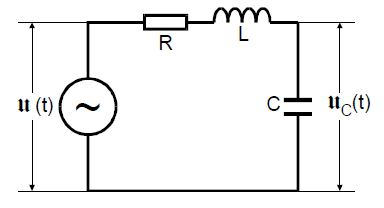
\includegraphics[height=5cm]{erzw.JPG}
  \caption{Schwingkreis mit äußerer Spannungsquelle}
  \cite{skript}.
  \label{fig:erzw}
\end{figure}
Die Differentialgleichung \ref{eqn:dgl} wird nun zu einer inhomogenen DGL der Form
\begin{equation}
  LC\ddot{U_{C}}+ RC\dot{U_{C}}+U_{C}=U_{0}e^{i\omega t}.
  \label{eqn:erzwdgl}
\end{equation}
Für die Spannung in Abhängigkeit der Zeit folgt daraus
\begin{equation}
  U(t)=\frac{U_{0}(1-LC\omega^2-i\omega RC)}{(1-LC\omega^2R^2C^2)}.
\end{equation}
Die Phasenverschiebung zur Erregerspannung ergibt sich durch vergleichen von
Real- und Imaginärteil:
\begin{equation}
  \Phi(t)=\arctan\Bigl(\frac{Im(U)}{Re(U)}\Bigr)=\arctan\Bigl(\frac{-\omega RC}{1-LC\omega^2}\Bigr).
\end{equation}

Die Spannung kann auch in Abhängigkeit der Frequenz $\omega$ angegeben werden
\begin{equation}
  U_{C}(\omega)=\frac{U_{0}}{\sqrt{(1-LC\omega^2)^2+\omega^2R^2C^2}}.
\end{equation}
Diese Funktion wird auch als Resonanzkurve bezeichnet. Für den Fall,
$\omega \to \infty$ geht $U_{C}$ gegen Null, während $U_{C}$ für
$\omega \to 0$ gegen die Erregeramplitude $U_{0}$ strebt.
Für eine "spezielle" Frequenz erreicht $U_{C}$ ein Maximun, dass größer
als $U_{0}$ sein kann. Diese Frequenz $\omega_{\text{res}}$ wird als Resonanzfrequenz
bezeichnet. Für sie gilt:
\begin{equation}
  \omega_{\text{res}}=\sqrt{\frac{1}{LC}-\frac{R^2}{2L^2}}.
  \label{eqn:res}
\end{equation}

Für den Spezialfall, dass
\begin{equation}
  \frac{R^2}{2L^2}<<\frac{1}{LC}
\end{equation}
gilt, wird von schwacher Dämpfung gesprochen. Für diesen Fall nähert sich
$\omega_{\text{res}}$ der Frequenz der ungedämpften Schwingung $\omega_{0}$.
Das Maximum der Kondensatorspannung ist für diesen Fall um den Faktor
\begin{equation}
  q=\frac{1}{\omega_{0}RC}
  \label{eqn:gute}
\end{equation}
größer als die Erregerspannung. Dieser Fakror $q$ wird als Güte des Schwingkreises
bezeichnet.



\label{sec:Theorie}

%\cite{sample}
||||||| merged common ancestors
\section{Theorie}
Im diesem Versuch wird der RLC-Schwingkreis untersucht, dieser besteht aus folgenden
Bauteilen: Widerstand $R$, Induktivität $L$ und Kondensator $C$.
Ähnlich zum RLC-Schingkreis ist der RC-Schwingkreis aufgebaut, er bestitzt nur einen
Energiespeicher, den Kondensator $C$.
Der RLC-Schwingkreis besitzt zwei Energiespeicher, einen Kondensator und eine
Spule. Wird nun Energie in das System hineingepumt, pendelt diese zwischen Kondensator und
Spule, wodurch der Strom sein Vorzeichen ändert. Der Widerstand, der hier dem
Dämpfungsfaktor entspricht, wandelt einen Teil der Energie in Wärme um. Nach einer
gewissen Zeitspanne ist keine elektrische Energie mehr vorhanden und die Schwingung
kommt zum erliegen. Dieses Verhalten wird auch als gedämpfte Schwingung bezeichnet.
Wenn kein Widerstand $R$ im System verbaut ist, wird dieses System als
ungedämpften Schwingung bezeichnet.
\begin{figure}[H]
  \centering
  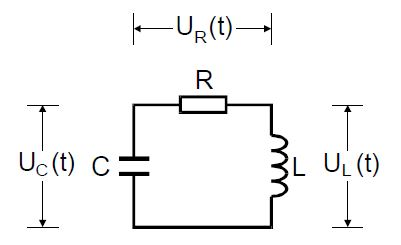
\includegraphics[height=5cm]{RLC.JPG}
  \caption{Darstellung eines RLC-Scwingkreises}
  \cite{skript}.
  \label{fig:RLC}
\end{figure}
Wird an den Schwingkreis von außen eine Spannung angelegt, schwingt dieser
mit der Frequenz der angelegten Spannung. Die so erhaltene Schwingung wird als
ezwungene Schwingung bezeichnet. Hat die von außen angelete Spannung die "richtige"
Frequenz (abhänging vom verwendeten System/Schwingkreis), dann erreicht die Stromamplitude im
Schwingkreis ihr Maximum. Dieser Fall wird als Resonanzfall bezeichnet und tritt bei der
sogenannten Resonanzfrequenz auf.

\subsection{Gedämpfte Schwingung}
In einem RLC-Schwingkreis, der wie in Abbildung \ref{fig:RLC} aufgebaut ist, gilt nach dem
2. Kirchfoffschen Gesetz:
\begin{equation}
  U_{R}(t)+U_{L}(t)+U_{C}(t)=0.
  \label{eqn:max}
\end{equation}
%Die Spannungen lassen sich auch wie folgt ausdrücken:
%\begin{align}
%  U_{R}&=RI\\
%  U_{C}&=\frac{Q(t)}{C}\\
%  U_{L}&=L\frac{dI}{dt}\\
%\text{außerdem gilt:}\:\:I&=\frac{dQ}{dt}.
%\end{align}
Ableiten nach der Zeit und umschreiben der Spanungen liefert dann die Differentialgleichung
für die gedämpfte Schwingung
\begin{equation}
  \ddot{I}+\frac{R}{L}\dot{I}+\frac{1}{LC}I=0.
  \label{eqn:dgl}
\end{equation}
Diese Differentialgleichung hat die allgemeine Lösung:
\begin{equation}
  I(t)=e^{-2 \pi\mu t}(A_{1}e^{2 \pi i \nu t}+A_{2}e^{-2\pi i \nu t})
  \label{eqn:lös}
\end{equation}
mit den Abkürzungen
\begin{align*}
  \mu = \frac{R}{4\pi L} \;\;\; \text{und}\\
  \nu=\frac{1}{2\pi}\sqrt{\frac{1}{LC}-\frac{R^2}{4L^2}}.
\end{align*}
Jetzt müssen noch folgende Fallunterscheidungen für ein reelles und ein
imaginäres $\nu$ getroffen weden:\\
1.Fall:\\
Wenn $\nu$ reell ist muss
\begin{equation}
  \frac{1}{LC}>\frac{R^2}{4L^2}
  \label{eqn:bed1}
\end{equation}
gelten, damit lässt sich Gleichung \ref{eqn:lös} zu
\begin{equation}
  I(t)=A_{0}e^{-2\pi \mu t}\cos(2\pi \nu t )
\end{equation}
umschreiben. Unter der Bedingung \ref{eqn:bed1} handelt es sich also um
eine gedämpfte Schwingung, da $I(t)$ für $t \to \infty$ gegen Null strebt.
Für die Abklingdauer gilt:
\begin{equation}
  T_{ex}=\frac{1}{2\pi \mu}.
  \label{eqn:tex}
\end{equation}\\
\\
2.Fall:\\
Wenn $\nu$ imaginär ist, muss
\begin{equation}
  \frac{1}{LC}<\frac{R^2}{4L^2}
  \label{bed2}
\end{equation}
gelten, damit kann Gleichung \ref{eqn:lös} zu
\begin{equation}
  I(t) \propto e^{-(2\pi \mu -2\pi i \nu)t}
\end{equation}
umgeformt werden. Da $\nu$ nun imaginär ist, kommen nur noch
reelle Exponenten vor und es gibt keinen oszillierenden Anteil mehr.
Dieser Fall wird aperiodische Dämpfung genannt.\\
\\
3.Fall:\\
Ein Spezialfall ist, wenn
\begin{equation}
  \frac{1}{LC}= \frac{R_{\text{ap}}^2}{4L^2}
  \label{eqn:bed3}
\end{equation}
gilt, also wenn $\nu=0$ ist.
Für den Strom folgt dann:
\begin{equation}
  I(t)=Ae^{\frac{-t}{\sqrt{LC}}}.
\end{equation}
Dieser Fall ist der aperiodische Grenzfall. $I(t)$ geht direkt, ohne
Überschwingen, gegen Null.\\
\\

\subsection{Erzwungene Schwingung}
Nun wird an den gedämpften Schwingkreis eine Spannungsquelle angeschlossen, die
eine Sinusförmige Wechselspannung $U_{S}=U_{0}e^{i\omega t}$ liefert.
\begin{figure}[H]
  \centering
  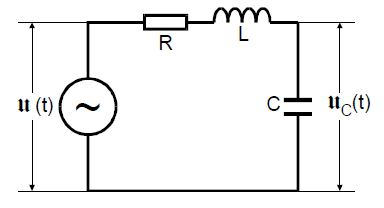
\includegraphics[height=5cm]{erzw.JPG}
  \caption{Schwingkreis mit äußerer Spannungsquelle}
  \cite{skript}.
  \label{fig:erzw}
\end{figure}
Die Differentialgleichung \ref{eqn:dgl} wird nun zu einer inhomogenen DGL der Form
\begin{equation}
  LC\ddot{U_{C}}+ RC\dot{U_{C}}+U_{C}=U_{0}e^{i\omega t}.
  \label{eqn:erzwdgl}
\end{equation}
Für die Spannung in Abhängigkeit der Zeit folgt daraus
\begin{equation}
  U(t)=\frac{U_{0}(1-LC\omega^2-i\omega RC)}{(1-LC\omega^2R^2C^2)}.
\end{equation}
Die Phasenverschiebung zur Erregerspannung ergibt sich durch vergleichen von
Real- und Imaginärteil:
\begin{equation}
  \Phi(t)=\arctan\Bigl(\frac{Im(U)}{Re(U)}\Bigr)=\arctan\Bigl(\frac{-\omega RC}{1-LC\omega^2}\Bigr).
\end{equation}

Die Spannung kann auch in Abhängigkeit der Frequenz $\omega$ angegeben werden
\begin{equation}
  U_{C}(\omega)=\frac{U_{0}}{\sqrt{(1-LC\omega^2)^2+\omega^2R^2C^2}}.
\end{equation}
Diese Funktion wird auch als Resonanzkurve bezeichnet. Für den Fall,
$\omega \to \infty$ geht $U_{C}$ gegen Null, während $U_{C}$ für
$\omega \to 0$ gegen die Erregeramplitude $U_{0}$ strebt.
Für eine "spezielle" Frequenz erreicht $U_{C}$ ein Maximun, dass größer
als $U_{0}$ sein kann. Diese Frequenz $\omega_{\text{res}}$ wird als Resonanzfrequenz
bezeichnet. Für sie gilt:
\begin{equation}
  \omega_{\text{res}}=\sqrt{\frac{1}{LC}-\frac{R^2}{2L^2}}.
\end{equation}

Für den Spezialfall, dass
\begin{equation}
  \frac{R^2}{2L^2}<<\frac{1}{LC}
\end{equation}
gilt, wird von schwacher Dämpfung gesprochen. Für diesen Fall nähert sich
$\omega_{\text{res}}$ der Frequenz der ungedämpften Schwingung $\omega_{0}$.
Das Maximum der Kondensatorspannung ist für diesen Fall um den Faktor
\begin{equation}
  q=\frac{1}{\omega_{0}RC}
  \label{eqn:gute}
\end{equation}
größer als die Erregerspannung. Dieser Fakror $q$ wird als Güte des Schwingkreises
bezeichnet.



\label{sec:Theorie}

%\cite{sample}
=======
\section{Theorie}
Im diesem Versuch wird der RLC-Schwingkreis untersucht, dieser besteht aus folgenden
Bauteilen: Widerstand $R$, Induktivität $L$ und Kondensator $C$.
Ähnlich zum RLC-Schingkreis ist der RC-Schwingkreis aufgebaut, er bestitzt nur einen
Energiespeicher, den Kondensator $C$.
Der RLC-Schwingkreis besitzt zwei Energiespeicher, einen Kondensator und eine
Spule. Wird nun Energie in das System hineingepumt, pendelt diese zwischen Kondensator und
Spule, wodurch der Strom sein Vorzeichen ändert. Der Widerstand, der hier dem
Dämpfungsfaktor entspricht, wandelt einen Teil der Energie in Wärme um. Nach einer
gewissen Zeitspanne ist keine elektrische Energie mehr vorhanden und die Schwingung
kommt zum erliegen. Dieses Verhalten wird auch als gedämpfte Schwingung bezeichnet.
Wenn kein Widerstand $R$ im System verbaut ist, wird dieses System als
ungedämpften Schwingung bezeichnet.
\begin{figure}[H]
  \centering
  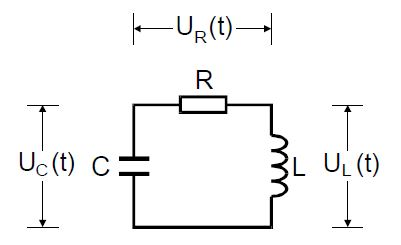
\includegraphics[height=5cm]{RLC.JPG}
  \caption{Darstellung eines RLC-Scwingkreises}
  \cite{skript}.
  \label{fig:RLC}
\end{figure}
Wird an den Schwingkreis von außen eine Spannung angelegt, schwingt dieser
mit der Frequenz der angelegten Spannung. Die so erhaltene Schwingung wird als
ezwungene Schwingung bezeichnet. Hat die von außen angelete Spannung die "richtige"
Frequenz (abhänging vom verwendeten System/Schwingkreis), dann erreicht die Stromamplitude im
Schwingkreis ihr Maximum. Dieser Fall wird als Resonanzfall bezeichnet und tritt bei der
sogenannten Resonanzfrequenz auf.

\subsection{Gedämpfte Schwingung}
In einem RLC-Schwingkreis, der wie in Abbildung \ref{fig:RLC} aufgebaut ist, gilt nach dem
2. Kirchfoffschen Gesetz:
\begin{equation}
  U_{R}(t)+U_{L}(t)+U_{C}(t)=0.
  \label{eqn:max}
\end{equation}
%Die Spannungen lassen sich auch wie folgt ausdrücken:
%\begin{align}
%  U_{R}&=RI\\
%  U_{C}&=\frac{Q(t)}{C}\\
%  U_{L}&=L\frac{dI}{dt}\\
%\text{außerdem gilt:}\:\:I&=\frac{dQ}{dt}.
%\end{align}
Ableiten nach der Zeit und umschreiben der Spanungen liefert dann die Differentialgleichung
für die gedämpfte Schwingung
\begin{equation}
  \ddot{I}+\frac{R}{L}\dot{I}+\frac{1}{LC}I=0.
  \label{eqn:dgl}
\end{equation}
Diese Differentialgleichung hat die allgemeine Lösung:
\begin{equation}
  I(t)=e^{-2 \pi\mu t}(A_{1}e^{2 \pi i \nu t}+A_{2}e^{-2\pi i \nu t})
  \label{eqn:lös}
\end{equation}
mit den Abkürzungen
\begin{align*}
  \mu = \frac{R}{4\pi L} \;\;\; \text{und}\\
  \nu=\frac{1}{2\pi}\sqrt{\frac{1}{LC}-\frac{R^2}{4L^2}}.
\end{align*}
Jetzt müssen noch folgende Fallunterscheidungen für ein reelles und ein
imaginäres $\nu$ getroffen weden:\\
1.Fall:\\
Wenn $\nu$ reell ist muss
\begin{equation}
  \frac{1}{LC}>\frac{R^2}{4L^2}
  \label{eqn:bed1}
\end{equation}
gelten, damit lässt sich Gleichung \ref{eqn:lös} zu
\begin{equation}
  I(t)=A_{0}e^{-2\pi \mu t}\cos(2\pi \nu t )
\end{equation}
umschreiben. Unter der Bedingung \ref{eqn:bed1} handelt es sich also um
eine gedämpfte Schwingung, da $I(t)$ für $t \to \infty$ gegen Null strebt.
Für die Abklingdauer gilt:
\begin{equation}
  T_{ex}=\frac{1}{2\pi \mu}.
  \label{eqn:tex}
\end{equation}\\
\\
2.Fall:\\
Wenn $\nu$ imaginär ist, muss
\begin{equation}
  \frac{1}{LC}<\frac{R^2}{4L^2}
  \label{bed2}
\end{equation}
gelten, damit kann Gleichung \ref{eqn:lös} zu
\begin{equation}
  I(t) \propto e^{-(2\pi \mu -2\pi i \nu)t}
\end{equation}
umgeformt werden. Da $\nu$ nun imaginär ist, kommen nur noch
reelle Exponenten vor und es gibt keinen oszillierenden Anteil mehr.
Dieser Fall wird aperiodische Dämpfung genannt.\\
\\
3.Fall:\\
Ein Spezialfall ist, wenn
\begin{equation}
  \frac{1}{LC}= \frac{R_{\text{ap}}^2}{4L^2}
  \label{eqn:bed3}
\end{equation}
gilt, also wenn $\nu=0$ ist.
Für den Strom folgt dann:
\begin{equation}
  I(t)=Ae^{\frac{-t}{\sqrt{LC}}}.
\end{equation}
Dieser Fall ist der aperiodische Grenzfall. $I(t)$ geht direkt, ohne
Überschwingen, gegen Null.\\
\\

\subsection{Erzwungene Schwingung}
Nun wird an den gedämpften Schwingkreis eine Spannungsquelle angeschlossen, die
eine Sinusförmige Wechselspannung $U_{S}=U_{0}e^{i\omega t}$ liefert.
\begin{figure}[H]
  \centering
  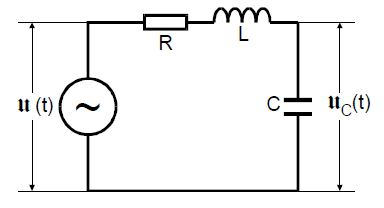
\includegraphics[height=5cm]{erzw.JPG}
  \caption{Schwingkreis mit äußerer Spannungsquelle}
  \cite{skript}.
  \label{fig:erzw}
\end{figure}
Die Differentialgleichung \ref{eqn:dgl} wird nun zu einer inhomogenen DGL der Form
\begin{equation}
  LC\ddot{U_{C}}+ RC\dot{U_{C}}+U_{C}=U_{0}e^{i\omega t}.
  \label{eqn:erzwdgl}
\end{equation}
Für die Spannung in Abhängigkeit der Zeit folgt daraus
\begin{equation}
  U(t)=\frac{U_{0}(1-LC\omega^2-i\omega RC)}{(1-LC\omega^2R^2C^2)}.
\end{equation}
Die Phasenverschiebung zur Erregerspannung ergibt sich durch vergleichen von
Real- und Imaginärteil:
\begin{equation}
  \Phi(t)=\arctan\Bigl(\frac{Im(U)}{Re(U)}\Bigr)=\arctan\Bigl(\frac{-\omega RC}{1-LC\omega^2}\Bigr).
\end{equation}

Die Spannung kann auch in Abhängigkeit der Frequenz $\omega$ angegeben werden
\begin{equation}
  U_{C}(\omega)=\frac{U_{0}}{\sqrt{(1-LC\omega^2)^2+\omega^2R^2C^2}}.
\end{equation}
Diese Funktion wird auch als Resonanzkurve bezeichnet. Für den Fall,
$\omega \to \infty$ geht $U_{C}$ gegen Null, während $U_{C}$ für
$\omega \to 0$ gegen die Erregeramplitude $U_{0}$ strebt.
Für eine "spezielle" Frequenz erreicht $U_{C}$ ein Maximun, dass größer
als $U_{0}$ sein kann. Diese Frequenz $\omega_{\text{res}}$ wird als Resonanzfrequenz
bezeichnet. Für sie gilt:
\begin{equation}
  \omega_{\text{res}}=\sqrt{\frac{1}{LC}-\frac{R^2}{2L^2}}.
\end{equation}

Für den Spezialfall, dass
\begin{equation}
  \frac{R^2}{2L^2}<<\frac{1}{LC}
\end{equation}
gilt, wird von schwacher Dämpfung gesprochen. Für diesen Fall nähert sich
$\omega_{\text{res}}$ der Frequenz der ungedämpften Schwingung $\omega_{0}$.
Das Maximum der Kondensatorspannung ist für diesen Fall um den Faktor
\begin{equation}
  q=\frac{1}{\omega_{0}RC}
  \label{eqn:gute}
\end{equation}
größer als die Erregerspannung. Dieser Fakror $q$ wird als Güte des Schwingkreises
bezeichnet.



\label{sec:Theorie}

%\cite{sample}
>>>>>>> michelson
